\begin{itemize}
\item Introduction for the implementation section.
\item Introduction should perhaps introduce the topics of this chapter.
\end{itemize}

\textbf{What is the implementation chapter about?}\\
This chapter delves into the development of 5 prototypes, each portraying a different type of behaviour for hands in VR. These different prototypes approach the problem of realism vs sense of embodiment in different ways and to different degrees. In the following sections, we will present a categorization of approaches that can be taken when implementing hands in VR, what effects these different approaches have and their pros and cons.

\textbf{What stuff did we use during the project?} (headset and control scheme, for instance)\\
All 5 prototypes have been developed using the Unity engine and the HTC Vive with default controllers for input. The space we've explored during the development of the prototypes have been restricted by these choices. Unity has a set of APIs which we as users of Unity have available to us. These APIs have shaped what has been possible for us during implementation of the prototypes. Furthermore, building the prototypes around using the HTC Vive's controllers as the input method makes our methods and approaches more applicable to hardware that has the same affordances as these. As for the input used to control the hands the position and orientation input is gathered from tracking the controllers and the controllers' trigger buttons are used to indicate how much the fingers should bend (how closed the hand should be).

\textbf{How does this lead into the categorizations?}\\
These three inputs are the base for different categories of approaches. Each of these inputs can be filtered, by which is meant that the input can be modified or skipped. Filtering on one of the inputs can be seen as using that input as the parameter for a function, which returns a new result. A hand can have a filter for either none of the inputs or one of the inputs or more. Different filtering combinations will give the hand a different behaviour in the virtual world and might result in the hand seeming more realistic when interacting with its environment.

The 5 hand prototypes are named as follows: \textit{Rigid hand}, \textit{Sliding rigid hand}, \textit{Finger rigid hand}, \textit{Physics hand} and \textit{Rotation hand}. They differ in the way they filter on the player's inputs which gives them a different feel. The detail of which filters and their implementation will be given in the sections below.

\todo[inline]{Maybe structure this chapter so that the different hand prototypes are introduced with their name before going into the specific filtering sections (for instance position filtering). Then inside the filtering sections the hands can be mentioned with their differences. After all the filter sections there can then perhaps be a section that reiterates over the hand prototypes and summarises their filtering implementations.}

\section{Categorization of approaches}
\label{sec:categorizationOfApproaches}
\begin{itemize}
\item Lead into the explanation for the filter variables.
\item Display filter variable table.
\item Describe several examples of filter variable combinations and show image sequences.
\item (Describe the reasons and effects for filtering on the different variables)?
\end{itemize}

The three player inputs mentioned above (position, orientation and how closed the hand should be) are the base of the categorization of approaches. Each of these inputs can be filtered, by which is meant that the input can be modified or skipped. Filtering on one of the inputs can be seen as using the input as the parameter for a function, which returns a new result which will be used instead of that input. A hand can be implemented with filters on several inputs at once and can have different filters depending on the context. Different filterer combinations will give a different behaviour for the hand in the virtual world and can result in the hand seeming more realistic when interacting with its environment.

\begin{table}[H]
\centering
\caption{Filter variable combinations.}
\label{tab:filterVariableCombinations}
\begin{tabular}{C{2cm}C{2cm}C{2cm}}
Position & Rotation & Finger position \\ \midrule \midrule
				&					&					\\ \midrule
\Large X	&					&					\\ \midrule
				& \Large X	& 		                \\ \midrule
				&					& \Large X     \\ \midrule
\Large X	& \Large X	&					\\ \midrule
\Large X 	&					& \Large X	\\ \midrule
				& \Large X	& \Large X	\\ \midrule
\Large X 	& \Large X 	& \Large X
\end{tabular}
\end{table}

\subsection{Position filtering}
\label{subsec:categoryPositionFiltering}
\textbf{Questions to answer in this section:}
\begin{itemize}
\item What does it mean to filter the player's positional input?
\item Why do we want to filter the player's positional input?
\end{itemize}

\textbf{What does it mean to filter the player's positional input?}\\
A position filter using the definition above is a function, which when enabled, takes the player's positional input from a controller and returns a new value to be used in its stead. This means that the position of the hand in the virtual world will deviate from the controller position.

\textbf{Why do we want to filter the player's positional input?}\\
One of our hypotheses is that it's possible to increase the player's sense of embodiment by simulating more realistic behaviour for hands around objects in the world. One of the first steps here is to not allow the hands to penetrate objects. By using position filtering to deviate the hand from the controller position when trying to penetrate an object, the hand can interact more realistically with the world.

The following two figures show an image sequence of a hand with no input filtering and an image sequence with a hand that uses position filtering. The second figure shows that the hand is stopping when it reaches the object, whereas in the first figure the hand moves through the object.

\begin{figure}[H]
\label{fig:filtersNone}
\centering
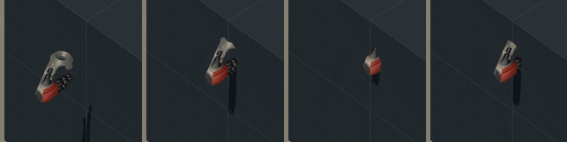
\includegraphics[width=\textwidth]{Sequences/FiltersNone/Seq_FiltersNone.png}
\caption{Sequence showing hand without filters entering obstacle.}
\end{figure}

\begin{figure}[H]
\label{fig:filtersPosition}
\centering
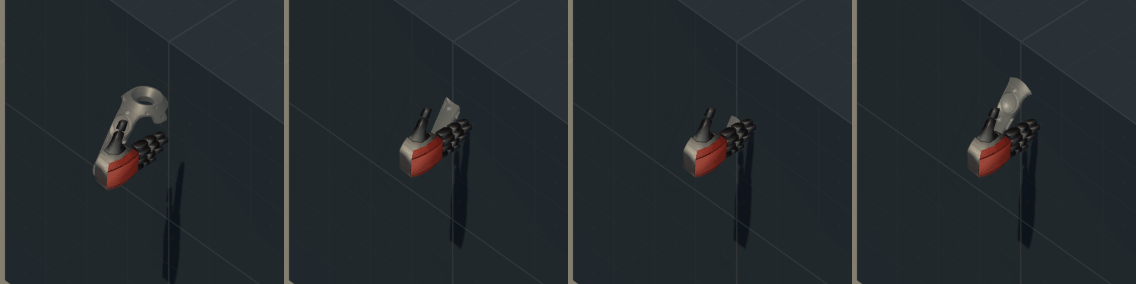
\includegraphics[width=\textwidth]{Sequences/FiltersPosition/Seq_FiltersPosition.png}
\caption{Sequence showing hand filtering on position. Notice the controller continuing to move into the obstacle.}
\end{figure}

\textbf{Questions to answer in this section:}
\begin{itemize}
\item How can we filter the player's positional input?
\begin{itemize}
\item Depenetration.
\item Physics system.
\item Different filter methods have different restrictions.
\end{itemize}
\end{itemize}

\textbf{How can we filter the player's positional input?}\\
Implementing position filtering for hands is about determining how to make the hand follow the controller. All of our 5 prototypes use position filtering, but the implementations of the filters differ. The first distinction is between physics bases and non-physics based methods. The physics hand is the only one of our prototypes that falls into the first category. The way the physics hand is moved towards the controller is to set the velocity each frame so that the hand will reach the controller within the next frame using the physics system. Using velocities and the physics system to move the hand has several positive aspects. The main gain of using the physics system to move is that it adheres to the rules of the system, including collisions, which means that the hand will not penetrate objects in the world which have colliders. Using the physics system to avoid penetration is very efficient since it's one of the core features of the Unity engine. One of the downsides of using the physics system to handle collisions and more is that we as the developers have no direct control over the inner workings of the system and therefore lose some control of how the hand behaves.

As for the prototypes that are implemented using non-physics based methods, their filters are all based on three different approaches to stop the hands from penetrating objects: Sweep and place, skip movement in direction and depenetration. These three methods fall into two categories; pre-collision correction methods and post-collision correction methods. The first two methods fall into the pre-collision correction category, because they try to avoid penetration of objects before it happens, whereas depenetration, which falls into the post-collision correction category will correct the penetration after it has happened. In the different prototypes these three methods are used alone or in combination to create the behaviour wanted from that prototype. The simplest of these prototypes is the Rigid hand. Here only the depenetration comes into play. Depenetrating the hand from an object means to find the direction and distance in which to move the colliders of the hand in order for the hand and the object not to be overlapping anymore. The direction is to the closest surface and the distance is the distance needed to move for the collider to be outside the object's colliders. When moving the hands in this prototype, their position is simply set to the target position on the controller each frame after which they are depenetrated from any objects they would be overlapping with. Using this method creates very smooth interactions with static objects, but have drawbacks for interacting with dynamic objects (EXPLAIN THESE DRAWBACKS). Since the hand is always depenetrated to the closest surface there is also the drawback of the hand jumping between surfaces, when the controller is places inside a static object. If in one frame the hand is closer to one surface and another surface in the next frame, depenetrating the hand from the object will lead it to move towards another surface creating a jump.

The problem of jumping between surfaces, when using depenetration is what the Sliding rigid hand is trying to solve. They employ the other two methods, Sweep and place and skip movement in direction, in order to combat the jumping between surfaces. The main idea behind this prototype is to try avoiding penetrating an object altogether or if it happens to only penetrate a small amount so that depenetrating the hand would always select the same surface from where it entered the object. Sweeping is about taking the hand and calculating how far in a direction it can move before it hits something. Before moving the hand to the controller position we can sweep and see if it would hit an object on the way. If an object was hit then the hand can be placed there instead of placing it at the controller. This way the hand will not penetrate the object although the controller is inside or on the opposite side of it. In Unity sweeping in a direction will not detect an object if the hand already touches the object. Therefore, in subsequent frames from placing the object on the surface, another method is needed for the hand to not penetrate the object. Skipping movement in a direction is one way to alleviate this problem. When the hand is touching the surface of an object, it shouldn't move in the direction towards the surface, because that would lead the hand to penetrate the object. Therefore, we skip all movement along that direction, essentially allowing the hand to only move on a plane. Moving on a plane works wonders, when interacting with cubes, but has its downsides, when dealing with objects with other shapes. Sliding on a plane might lead the hand to penetrate parts of an object that point out or penetrate other objects. Depenetration helps correct the hands in the situations, where they end up inside an object because correcting in one way leads to errors some place else. These three methods combined should lead to hands that don't penetrate objects, but also doesn't jump between surfaces due to depenetration.

The two remaining prototypes, the Finger rigid hand and the Rotation hand, both use the methods mentioned above to achieve their position filtering. The Finger rigid hand use the exact same position filtering method as the Rigid hands and the Rotation hand use a filter similar to the Sliding rigid hand with the exception that it doesn't do any depenetration.

\subsection{Rotation filtering}
\label{subsec:categoryRotationFiltering}
\textbf{Questions to answer in this section:}
\todo{Alternative term: orientation}
\begin{itemize}
\item What does it mean to filter the player's rotational input?
\item Why do we want to filter the player's rotational input?
\begin{itemize}
\item Reduce position filtering.
\item Display player's intentions.
\item Diagetically communicate available interactions.
\item Allows for more detailed hand animation depending on available interactions. Control?
\item Mention stiffness with only position filtering
\end{itemize}
\end{itemize}

\textbf{What does it mean to filter the player's rotational input?}\\
To use a rotation filter is to deviate the hands rotation from the current orientation of the controller. In certain contexts it can be beneficial filter on rotation on order for the hand to seem more alive and realistic. Hands can adapt their rotation in several ways and different approaches might be taken depending on the context. When approaching a wall with their hand a player's intention in the real world might be to place their hand flat on the wall (palm-first). This behaviour can be implemented using a rotation filter, which takes effect when the hand is approaching a surface.

\textbf{Why do we want to filter the player's rotational input?}\\
Rotation filtering can be used to display what is assumed to be the player's intention when they interact with the world. One example could be the intention of the player when they approach a wall with their hand. In this case a reasonable assumption would be that the player's intention is to rotate the hand so that the palm faces the wall (See image sequences below). Besides being useful when wanting to adapt the hand to the player's intentions, rotation filtering can also be used in order to reduce the amount of position filtering needed. This means that rotating the hand will allow the distance between the hand and the controller due to position adjusting to be reduced (See image sequence below).

\todo[inline]{use refs}
The first of the two figures below shows an image sequence of a hand using only rotation filtering and the second figure shows an image sequence of a hand using both position and rotation filtering where the rotation filtering is implemented as palm-first towards the surface.

\missingfigure[figwidth=15cm]{Image sequence: Rotation filtering}
\missingfigure[figwidth=15cm]{Image sequence: Position and rotation filtering}

\textbf{Questions to answer in this section:}
\begin{itemize}
\item How can we filter the player's rotational input?
\begin{itemize}
\item Manual rotation filtering when approaching obstacles.
\item Differentiation between object types and angles of approach.
\item Physics system.
\end{itemize}
\end{itemize}

\todo[inline]{Remember explicit vs implicit rotation filtering (explicit being where we completely control the rotation vs the for instance the physics system controlling it).}

\textbf{How can we filter the player's rotational input?}\\
Although all our hand prototypes use position filters, only 2 of our 5 hand prototypes (Physics hand and Rotation hand) use rotation filtering.

For the physics hand, we don't use any explicit rotation filtering. The physics system decides the rotation of the hand, when interacting with surfaces. While the controller is within an object, the physics hand can decide to rotate the hand to a flat position (either palm-up or palm-down) in order to reduce the position deviation between the hand and the controller. The rotation happens as a jump and not as a smooth movement towards the surface resulting in a less natural feel during the jump, but a somewhat realistic look afterwards. To improve upon this, explicit rotation filtering could have been added to smoothly rotate the hand to lay flat on the surface, which could remove the jump altogether, but at the same time introduce complexity to the implementation.

Contrary to the physics hand the Rotation hand uses explicit rotation filtering. The goal of the rotation filtering for this hand was to always approach a surface palm-first. The main example to explain this choice is the approach of a hand towards a wall. When a player wants to put their hand on a wall, which way would they want to do this? Having an open hand and moving the hand fingers first wouldn't make much sense. It would not give support if the reason for touching the wall was to lean against it, for instance. Rotating the hand so that the palm would be placed firmly on the surface of the wall would make more sense in this case. With this as the main idea behind the rotation, the implementation then had to support this in several cases. The easy case is when the player approaches the wall with an open hand and the palm being closer to the surface than the back of the hand. Depending on the distance to the surface we rotate the palm of the hand the rest of the way until it is directly facing the surface. Another case is what to do when the hand is closed into a fist. In this case, the player is probably trying to punch the wall, which means that the palm shouldn't be facing the wall. Testing for this case isn't necessarily hard in itself, but other cases pile on top of this, including what to do when approaching with the back of the hand, what to do when the player is rotating while the hand is touching the surface and more.

\subsection{Finger position filtering}
\label{subsec:categoryFingerFiltering}
\textbf{Questions to answer in this section:}
\begin{itemize}
\item What does it mean to filter the player's finger position input?
\item Why do we want to filter the player's finger position input?
\begin{itemize}
\item Reduce position filtering.
\item Display player's intention.
\end{itemize}
\end{itemize}

\textbf{What does it mean to filter the player's finger position input?}\\
Filtering the finger positions is about placing the finger tips in space relatively to the rest of the hand or put differently; stretching and bending the fingers. The fingers can be filtered as a group or individually and different contexts can determine different filters.

\textbf{Why do we want to filter the player's finger position input?}\\
Here, like with the rotation filtering, a certain amount of assumptions have to be made about what the player's intend is. When a player's hand is approaching an object that can be grabbed, the most common case might be that they are trying to grab the object. If this is the case, adjusting the fingers to form a grip could be a natural behaviour.

\missingfigure[figwidth=15cm]{Image sequence: Position and finger position filtering}

\textbf{Questions to answer in this section:}
\begin{itemize}
\item How can we filter the player's finger position input?
\begin{itemize}
\item Filtering to avoid obstacles.
\item Filtering to anticipate player intent.
\item Differentiation between object types and angles of approach.
\end{itemize}
\end{itemize}

\textbf{How can we filter the player's finger position input?}\\
Implementations of finger position filtering include using an animation system to animate the fingers together or individually to different poses and the use of an Inverse Kinematics (IK) system to infer finger pose from finger tip position and hand position and orientation.

\todo[inline]{Obviously you skipped the actual methods?}

\section{The hand prototypes}
\label{sec:theHandPrototypes}
\begin{itemize}
\item Introduction to this section.
\item Describe each hand in detail referring to the filter methods mentioned in the above section.
\item This section should also describe the setup of the hands and can go into Unity specifics if needed.
\item Mention the controller target position and rotation.
\end{itemize}

\begin{table}[H]
\centering
\caption{The hand prototypes and their filters.}
\label{tab:handPrototypes}
\begin{tabular}{C{2.8cm}|C{2cm}C{2cm}C{2cm}C{2cm}C{2cm}}
 & Rigid hand & Sliding rigid hand & Finger rigid hand & Physics hand & Rotation hand \\ \midrule
Position filter & \Large X & \Large X & \Large X & \Large X & \Large X\\ \midrule
Rotation filter & & & & \Large X & \Large X \\ \midrule
Finger position Filter & & & \Large X & \Large X & \Large X 
\end{tabular}
\end{table}

\subsection{The Rigid hand}
\label{subsec:theRigidHand}
The process of creating the Rigid hand starts with setting up colliders for the model. In our case, we used a box collider for the palm of the hand and one for each part of each finger. It's important to make sure that the colliders are not able to collide and interact with each other. In Unity we made all colliders reside on a specific layer and made the physics system ignore interactions between objects within that layer. If this is not done, the hand might collide with itself and disallow fingers from bending etc. Furthermore, to allow us to use methods like sweep casting in Unity, the hand also needs a kinematic rigidbody. The rigidbody needs to be kinematic, because the physics system shouldn't handle collisions for the Rigid hand. In order to be able to close the fingers the Rigid hand also needs an animation which has two frames: An open hand and a closed hand. The trigger value from the controller can be used to blend between the two frames allowing the player to open and close their hand.

As mentioned above, the Rigid hand moves by setting the rigidbody's position and rotation to the selected position and rotation on the controller. In the case of moving the hand freely around without any collisions occurring the hand just follows the controller. In the case where the hand has penetrated one or more objects we will depenetrate it from the object. To detect if the hand needs to be depenetrated, we need to check if there is an overlap between the hand's colliders and any other colliders in the world. To reduce the number of colliders to check, we first find all colliders within a radius of the hand. Having these colliders we can now check if any of the hand's colliders have penetrated one or more of them. Unity's Physics API allows us to compute the penetration\footnote{Unity API: Physics.ComputePenetration(...)} between two colliders, which gives us the depenetration direction and distance. Iterating over all colliders in both the hand and the penetrated object, we can use the information gathered to move the hand out of the object, correcting the penetration error.

\begin{figure}[H]
\label{fig:stepByStepRigidHand}
\centering
\small
\begin{enumerate}
\item Move the hand's rigidbody to the target controller.
\item Orient the hand's rigidbody compared to the target controller.
\item Find all colliders within a small radius of the hand.
\item Compute if any of the found colliders are penetrated by one of the hand's colliders.
\item Depenetrate the hand based on the penetration information computed in the previous step.
\end{enumerate}
\caption{Step-by-step process for moving the Rigid hand.}
\end{figure}


\section{Miscellaneous shitz}
\label{sec:MISCELLANEOUSSHITZ}

\subsection{Hand visualization}
\label{subsec:handVisualization}

\subsection{Rumblez!}
\label{subsec:RUMLBEZ}

\subsection{Grabbing system details}
\label{subsec:grabbingSystem}